%\documentclass[10pt,preprint]{aastex}

\documentclass[10pt, a4paper, oneside]{article}

\usepackage[top=0cm, bottom=7cm, left=2cm, right=2cm]{geometry}

\usepackage{pdfpages}

\usepackage{hyperref}

\usepackage{color}


\textfloatsep 8.0pt


\usepackage[small,compact,center]{titlesec}

\setlength{\topmargin}{1pt}%	(gap above headers)
\setlength{\topskip}{1pt}	%	(between header and text}

\setlength{\parsep}{10pt}	%	(gap between paragraphs)
\setlength{\parindent}{20pt}	%	(indentation of paragraphs)

\setlength{\floatsep}{2pt} 	%	(space between floats (eg figures))
\setlength{\textfloatsep}{20pt}%	(space between floats and text)
\setlength{\abovecaptionskip}{2pt}	%(space above caption)
\setlength{\belowcaptionskip}{2pt}	%(space below caption)


\usepackage{subfigure}
\usepackage{natbib}
\usepackage{graphics}
\usepackage{graphicx}
\usepackage[outercaption]{sidecap}

\usepackage{wrapfig}




\begin{document}


\pagenumbering{roman}

\setcounter{page}{-1}






\section*{\sc \Large HELCATS Work Package 2: Description of Catalogue}

 
 \begin{center}
\begin{tabular}{ll}
\large Written by J.P. Byrne 	\hfill (RAL Space)
\end{tabular}
 \end{center}

\vskip 0.1 in


\pagenumbering{arabic}

\setcounter{page}{1}



This WP provides the foundation for the project, through the production of a catalogue of CMEs in the heliosphere. The catalogue is produced from manual inspection of STEREO/HI data (Task 1, outlined here: \href{http://www.helcats-fp7.eu/overview/activities_WP2}{http://www.helcats-fp7.eu/overview/activities\_WP2}). The resulting catalog is presented in Fig.~\ref{catalogue} below with a description of the parameters, followed by a series of three example CME observations in HI1 (Figs.~\ref{good}\,--\,\ref{poor}). 

Figure~\ref{catalogue} shows a screen-grab of the WP2 catalogue on the HELCATS website. The user may specify parameters for their search based on the `Date range' and the position angle on the plane-of-sky (`PA mid' \textcolor{red}{[Note: should this be PA fit?]} refers to the CME apex, while `PA width' refers the the CME span which is the difference between PA-North and PA-South). The columns of the catalogue are as follows:

\begin{enumerate}
\item {\bf ID}: The unique identifier for the observed CME.
\item {\bf Date [UTC]}: The date and time of the first observation of the CME in HI1.
\item {\bf SC}: The observing STEREO spacecraft, Ahead or Behind.
\item {\bf GT}: The `greater than' indicator for a CME than extends beyond the northern edge of the field-of-view. \textcolor{red}{[Note: the order of GT and LT need to be swapped]}
\item {\bf PA-N [deg]}: The most northern position angle of the CME span.
\item {\bf LT}: The `less than' indicator for a CME than extends beyond the southern edge of the field-of-view.
\item {\bf PA-S [deg]}: The most southern position angle of the CME span.
\item {\bf Quality}: A measure of Good, Fair or Poor, that indicates the quality of the CME observation and confidence that the eruption is by definition a CME.
\item {\bf PA fit [deg]}: The position angle used to perform a height-time fit to the CME.
\end{enumerate}


\begin{figure}[ht]
\centering{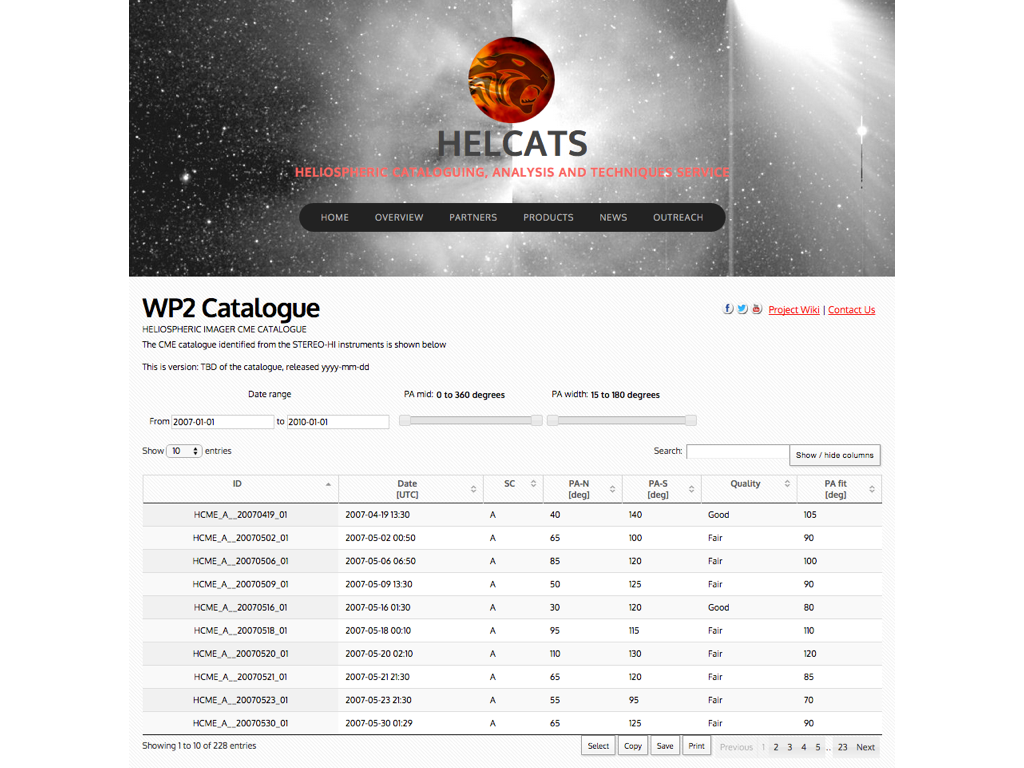
\includegraphics[width=\linewidth]{WP2_manualcatalog_images/WP2_manualcatalog_images008.png}}
\caption{\textcolor{red}{[Note: New screen-grab required]} A screenshot of the WP2 CME Catalogue, containing the parameters of the CMEs that were manually identified in the HI1 observations (listed in the text). Example CMEs from the catalogue are shown in Figs.\,\ref{good}--\,\ref{poor}.}
\label{catalogue}
\end{figure}


Figures~\ref{good}\,--\,\ref{poor} show three example CMEs, as viewed from the STEREO-Ahead spacecraft in February 2010. In each case the images have been processed to level 1 quality science data, a background has been subtracted, and a running-difference technique applied. CMEs therefor appear as bright regions propagating outward from the Sun (located at 0 degrees elongation). The chosen images list the time of the observation, the spacecraft longitude in Heliocentric Earth Ecliptic coordinates (HEE), the Earth's position angle, and the names of the fits file used in the running-difference subtraction. Overlaid on each image is a set of three arrows drawn to indicate (1) the angular width of the CME (blue arrows) and (2) its so-called central angle (red arrow) which is chosen as the best proxy for fitting the height-time profile of the CME.

\begin{figure}[ht]
\centering{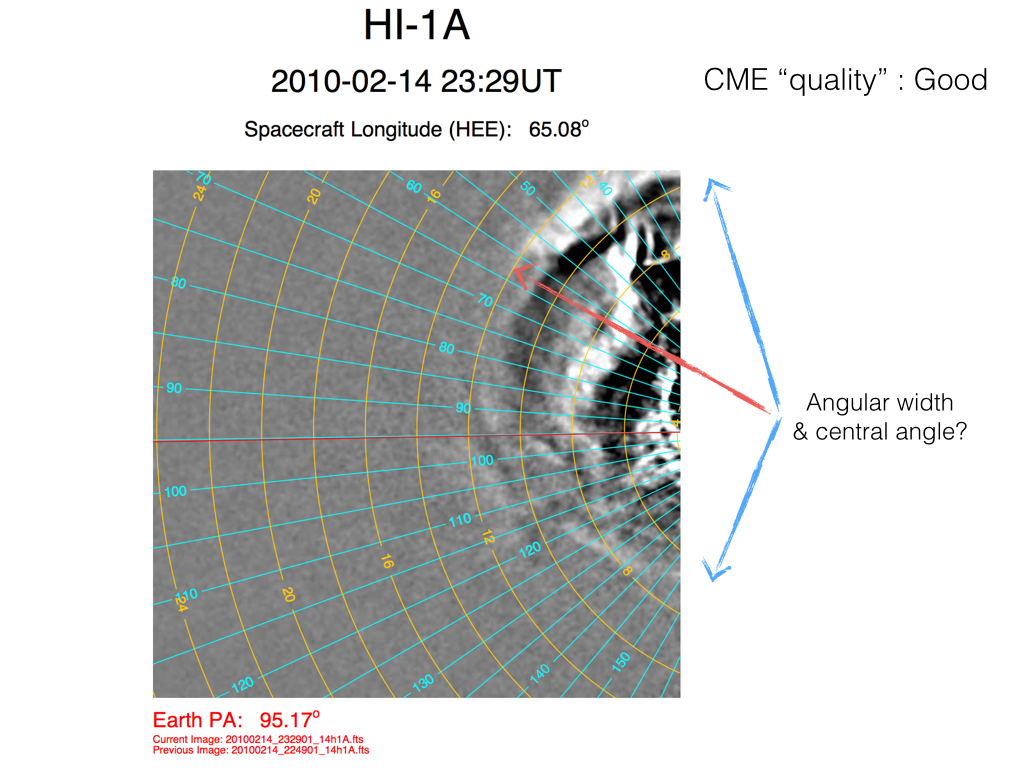
\includegraphics[width=\linewidth]{WP2_manualcatalog_images/WP2_manualcatalog_images003.png}}
\caption{An example CME observation with quality label `Good', on 14\,Feb.\,2010 seen in HI-1 from STEREO-Ahead. The angular width of the CME extends beyond the plane-of-sky as the CME propagates (blue arrows), so the central angle may be chosen close to 60 degrees (red arrow).}
\label{good}
\end{figure}



\begin{figure}[ht]
\centering{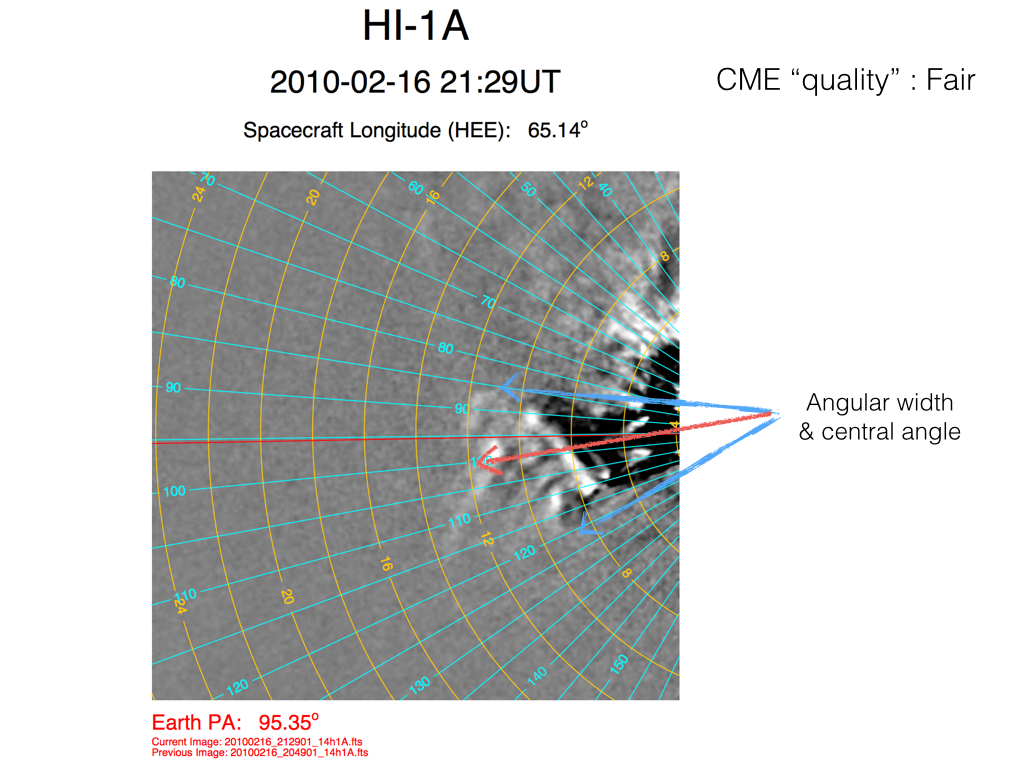
\includegraphics[width=\linewidth]{WP2_manualcatalog_images/WP2_manualcatalog_images005.png}}
\caption{An example CME observation with quality label `Fair', on 16\,Feb.\,2010 seen in HI-1 from STEREO-Ahead. The angular width of the CME extends from approximately 85\,--\,120 degrees (blue arrows), with an optimum central angle chosen around 100 degrees (red arrow).}
\label{fair}
\end{figure}



\begin{figure}[ht]
\centering{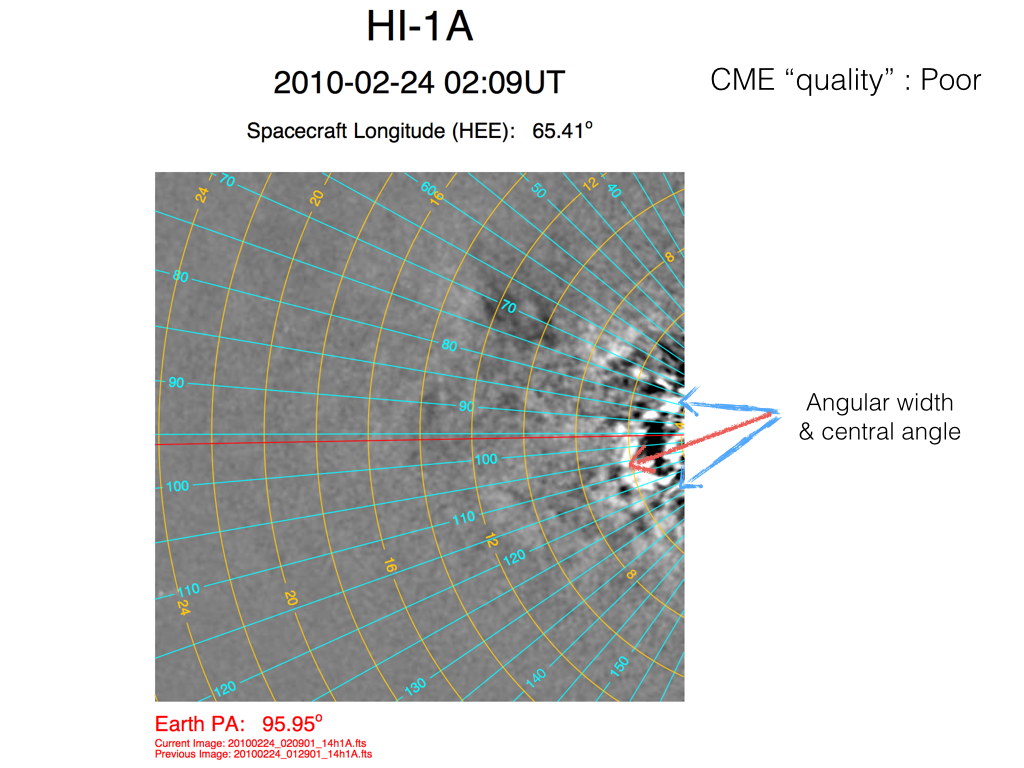
\includegraphics[width=\linewidth]{WP2_manualcatalog_images/WP2_manualcatalog_images007.png}}
\caption{An example CME observation with quality label `Poor', on 24\,Feb.\,2010 seen in HI-1 from STEREO-Ahead. The angular width of the CME extends from approximately 80\,--\,120 degrees (blue arrows), with an optimum central angle chosen around 105 degrees (red arrow).}
\label{poor}
\end{figure}








\end{document}
